
\documentclass{beamer}
\usepackage{changepage}
\usepackage{lmodern}
\usetheme{default}
\usepackage{listings}

\title{ROS Publisher/Subscriber Model}

\author{Kiran Vasudev\inst{1}}

\institute[] 
{
  \inst{1}
  Hochschule Bonn-Rhein-Sieg

}

\begin{document}

\begin{frame}
  \titlepage
\end{frame}

\begin{frame}{Outline}
  \tableofcontents
\end{frame}

\begin{frame}{The Publisher/Subscriber Pattern}
\section{The Publisher/Subscriber Pattern}
  \begin{itemize}
  \item {
	Transport system used to route messages
  }
  \item {
	A node sends a message by publishing it to a topic
  }
  \item {A node that is interested to access/use data certain data will subscribe to the most appropriate topic}
  \item{There can be many existing publishers and subscribers for a single topic}
  \item{A single node can publish/subscribe to multiple topics}
  \end{itemize}
\end{frame}

\begin{frame}
	\begin{figure}
		\begin{center}
			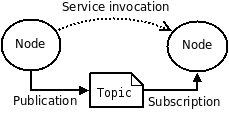
\includegraphics[scale=0.8]{images/basic_ros}
			\caption{The publish/subscribe model [1]}	
		\end{center}
	\end{figure}
\end{frame}


\begin{frame}{Cons of the Publisher/Subscriber Pattern}
\section{Cons of the Publisher/Subscriber Pattern}
  \begin{itemize}
  \item {
    The model's many-to-many one-way transport of messages are not appropriate for interactions based on requests/replies.
  }
  \item {   
    This con is overcome by using services (Will be introduced in the next session)
  }	
  \end{itemize}

\end{frame}

\begin{frame}[fragile]{Initializing a publisher and subscriber}
\section{Important commands}
\begin{itemize}
	\item {Python\\
	\begin{itemize}
		\item{\textbf{Publisher}}\\
		\footnotesize{pub = rospy.Publisher('chatter', String, queue\_size=10)}	\\
		\footnotesize{pub.publish(msg)}	\\
		
		\item{\textbf{Subscriber}}\\
		\footnotesize{rospy.Subscriber("chatter", String, callback)}	
	\end{itemize}
	}

	\item {C++ \\	
	\begin{itemize}
		\item{\textbf{Publisher}}\\
		\footnotesize{ros::Publisher chatter\_pub = n.advertise$\langle$std\_msgs::String $\rangle$("chatter", 1000);}	\\
		\footnotesize{chatter\_pub.publish(msg);}
		
		\item{\textbf{Subscriber}}\\
		\footnotesize{ros::Subscriber sub = n.subscribe("chatter", 1000, chatterCallback);}	
	\end{itemize}
}
\end{itemize}
\end{frame}	

\begin{frame}{Task}
	\section{Task}
	\begin{itemize}
		\item Create a new ROS package that has a minimum of two nodes: A publisher and a subscriber
		\item Define a custom message that contains:
		\begin{itemize}
			\item Image data
			\item LaserScan
			\item Pose 
		\end{itemize}
		Documentation to create a custom message is found here: 
	    \textbf{\href{http://wiki.ros.org/ROS/Tutorials/CreatingMsgAndSrv}{Creating messages}}
	    
		Use the documentation of ROS to define the message type. For example, the documentation of the sensor\_msgs can be found here: \textbf{\href{http://docs.ros.org/api/sensor_msgs/html/index-msg.html}{Sensor messages}}
		\item Play the given rosbag[4] and subscribe to the required topics for your new message in the subscriber node
		\item Using this information from the bag file, create your new message and publish it
		\item Once the message is published, subscribe to this message, and display a confirmation message once it has been received
	\end{itemize}
\end{frame}

\begin{frame}{Messages in ROS and their importance}
	\section{Messages in ROS and their importance}
	\begin{itemize}
		\item Nodes communicate with each other with the help of messages that are published to topics
		\item It is a data structure comprising of typed fields(int, float, boolean, arrays, etc.)
		\item Stored in the msg subdirectory of a package
		\item Naming convention:\\ \textbf{the name of the package + / + name of the .msg file \\ Example:  std\_msgs/String}
		\item It is used to generate source code for the type of message among different languages.
	\end{itemize}
\end{frame}

\begin{frame}{References}
	\section{References}
	\begin{enumerate}
		\item {\href{http://wiki.ros.org/custom/images/wiki/ROS_basic_concepts.png}{ROS Wiki}}
		\item {\href{http://wiki.ros.org/rospy/Overview/}{Publisher/Subscriber(python)}}
		\item {\href{http://wiki.ros.org/roscpp/Overview}{Publisher/Subscriber(cpp)}}
		\item{\href{http://projects.csail.mit.edu/stata/downloads.php}{ROSbag file}}
	\end{enumerate}
\end{frame}

\end{document}


